% --
% Master thesis main

\documentclass[twoside,openright]{scrreprt}
%\documentclass[report,mono,twoside,openright]{tugrazbooklet}
%\documentclass[a4paper]{book}

% added package prior to thesis
\usepackage[table]{xcolor}

% tu stuff
\usepackage[msc]{tugrazthesis}

% Example packages for the dummy content
%\usepackage{blindtext}


% --
% bib
\usepackage[backend=biber,style=alphabetic]{biblatex}

% add my bib
\addbibresource{bibl.bib}


% --
% my packages, macros and colors

% --
% added packages

\usepackage{array}
\usepackage{float}
\usepackage{tikz}
\usepackage{multirow} 
\usepackage{amssymb}
\usepackage{amsmath}
\usepackage{amsfonts} 
\usepackage{mathrsfs}
\usepackage{geometry}
\usepackage{graphicx}
\usepackage{siunitx}
\usepackage{tabularx}
\usepackage{caption}
\usepackage{subfigure}
\usepackage{rotating}
\usepackage{enumitem}
\usepackage{flafter}
\usepackage{placeins}
\usepackage{float}
\usepackage{psfrag}
\usepackage{wrapfig}
\usepackage[colorlinks=false, allcolors=blue]{hyperref}
\usepackage{csquotes}
\usepackage{commath}
\usepackage{booktabs}

% font and beautiful letters
\usepackage{yfonts}

% --
% Macros

%{A reference to Figure~\ref{fig:dummy}, Table~\ref{tab:dummy}, and a book \cite{Knuth97}.}

% refs
\newcommand{\rchp}[1]{Chapter~\ref{chp:#1}} 
\newcommand{\rchps}[1]{Chapters~\ref{chp:#1}} 
\newcommand{\rsec}[1]{Section~\ref{sec:#1}} 
\newcommand{\rsecs}[1]{Sections~\ref{sec:#1}} 
\newcommand{\rappendix}[1]{Appendix~\ref{#1}} 
\newcommand{\rfig}[1]{Figure~\ref{fig:#1}} 
\newcommand{\rfigs}[1]{Figures~\ref{fig:#1}} 
\newcommand{\rtab}[1]{Table~\ref{tab:#1}} 
\newcommand{\rtabs}[1]{Tables~\ref{tab:#1}} 
\newcommand{\rlst}[1]{Listing~\ref{lst:#1}} 
\newcommand{\rlsts}[1]{Listings.~\ref{lst:#1}} \newcommand{\req}[1]{(\ref{eq:#1})}

% math
\newcommand{\R}{\mathbb{R}}
\newcommand{\N}{\mathbb{N}}
\newcommand{\E}{\mathbb{E}}
\newcommand{\C}{\mathbb{C}}
\newcommand{\lam}{\lambda}
\newcommand{\g}{\nabla}
\newcommand{\inner}[2]{\langle #1, #2\rangle}
\newcommand{\sign}[1]{\mathrm{sgn}(#1)}
\newcommand{\interior}{\mathrm{int}}
\newcommand{\domain}{\mathrm{dom}}
\newcommand{\gradx}[1]{\begin{pmatrix} \frac{\partial}{\partial #1_1}\\\vdots\\\frac{\partial}{\partial #1_n}\end{pmatrix}}
\newcommand{\partialx}[1]{\frac{\partial}{\partial x_{#1}}}
\newcommand{\ball}[1]{B_{\norm{\cdot}_\infty}[0, #1]}
\newcommand{\deltaBall}[1]{\delta_{B_{\norm{\cdot}_\infty}[0, #1]}}
\newcommand{\proxMap}[2]{\mathrm{prox}_{#1 #2}}
\newcommand{\mor}{\frac{1}{2 \lambda} \norm{x-y}^2}
\newcommand{\diag}[1]{\mathrm{diag(#1)\,}}
\newcommand{\id}{\mathrm{\,Id\,}}
\newcommand{\proj}[1]{\mathrm{proj}_{#1}}
\newcommand{\prox}[1]{\mathrm{prox}_{#1}}

% tables
\newcolumntype{M}[1]{>{\centering\arraybackslash}m{#1}}

% booktabs tables
\setlength{\heavyrulewidth}{1.5pt}
\setlength{\abovetopsep}{4pt}
% --
% colors


% unused
\definecolor{LightYellow}{HTML}{ffff99}

% 
\definecolor{ThesisColor}{HTML}{aabb99}


% --
% begin document

\begin{document}

% myself
\thesisauthor[Christian Walter]{Christian Walter, BSc}

% thesis title
\thesistitle[Short Thesis Title]{Key Word Spotting for Video Games\\with Neural Networks}

% Date of completion (optional argument sets a different \date{})
\thesisdate[ ]{Month Year}

% Supervisor headline (select male/female/plural version)
\supervisortitle{\germanenglish{Betreuerin/Betreuer}{Supervisor}}

% Supervisor info
\supervisor{Robert Legenstein, Univ.-Prof. Dipl.-Ing. Dr.techn.\\Institute of Theoretical Computer Science\\}

% Academic degree achieved with this thesis, according to your curriculum (check curriculum and select male/female version):
\academicdegree{Master of Science}

% curriculum
\curriculum{Individuelles Masterstudium}
%\curriculum{Information and Computer Engineering } % 411
%\curriculum{Computer Science } % 921


% --
% titles

% title page
\printthesistitle

% affidavit
\printaffidavit

% abstract en
\chapter*{Abstract}
% --
% abstract

Key Word Spotting is a valuable tool in the interaction between humans and machines in various situations.
This thesis is specialised on the domain of Video Games and evaluates possible neural network architectures for speech command classifications tasks.
In focus are Convolutional Neural Network (CNN) architectures with adversarial pre-training using Mel Frequency Cepstral Coefficients (MFCC) as input features and Wavenets applied on raw audio samples.
The energy consumption and efficients is important in video games and therefore a strong criterion within this thesis.
Further some possible video game ideas or scenarios with speech command inputs with the purpose of triggering events within the games are evaluated and discussed.

% abstract de
\chapter*{Kurzfassung}
% --
% deutscher abstract

Deutsche Kurzfassung der Abschlussarbeit
\cleardoublepage

% Acknowledgement
\chapter*{\germanenglish{Danksagung}{Acknowledgements}}
% --
% Ack

Thanks to everyone who made this thesis possible.
\cleardoublepage

% table of contents
\tableofcontents
\listoffigures
\listoftables

% acronyms
\chapter*{\germanenglish{Abk\"{u}rzungs- und Symbolverzeichnis}{List of Acronyms and Symbols}}
KWS - Key Word Spotting\\
STFT - Short-Time Fourier Transform\\
DTFT - Discrete-Time Fourier Transform\\
DCT - Discrete Cosine Transform\\
MFCC - Mel Frequency Cepstral Coefficients\\
FPS - Frames Per Second\\
ASR - Automatic Speech Recognition\\
IPA - International Phonetic Alphabet\\


% -- 
% content

\chapter{Introduction}
Key Word Spotting is the task of identifying spoken words from human speakers out of a limited vocabulary or set of Key Words, e.g. identify the word \enquote{left} out of the vocabulary \{\enquote{left}, \enquote{right}\}. This problem is easily solved by humans in everyday live, but it is a real challenge for computer systems on which we aim to tackle it.

One approach to solve Key Word Spotting on a computer system is to use the advances of Machine Learning. which enables the computer to automatically learn abstract representations of the data given as input. 
The output of a Machine Learning system is...
and to infer an appropriate output, e.g. the waveform of \enquote{left} stored as \textit{.mp4} file is

Nowadays there are already many existing applications in the real world accessible for consumers (e.g. \textit{Alexa} from the company \textit{Amazon}).

While the task of Key Word Spotting is not a new one, it is solved with a variety of different approaches. One approach commonly used in recent times, is a Machine Learning system composed of a Neural Networks. The big advantage of Neural Networks is that they are able to learn how to process features in an automatic fashion, which means, that they learn their own feature extractions, selection and interpretation by themselves, rather than using hand-crafted ones done by humans with expertise in the application. 
What sound great at first hand, is also a bit of a downfall, as everyone who is able to use Machine Learning tools, can create a solution to rather complex problem usually done by experts, given they have enough data and processing power.
This solution concept therefore yield into less understanding of the actual problem and \enquote{try and error} approaches. However it is not always this way, certainly we can investigate how and why Neural Networks are able to produce such good results and therefore we might learn more on the field of expertise.

%However unfortunately due to the (usually) large amount of data and complex Neural Network Architectures it is in most cases not tractable, how these systems learn to distinguish between different samples. Nevertheless the technical benefits and their performance made them a standard tool in modern Machine Learning tasks.

\section{The task of Key Word Spotting}

We may define Key Word Spotting (KWS) as the task of classifying...
\section{Neural Networks for Automatic Speech Recognition}
Neural Networks for Automatic Speech Recognition must be discussed in a separate section, because there many different solution concepts for Key Word Spotting tasks and Neural Networks are just a subset of this solutions, yet a very powerful and modern one. Also there exist a large variety of different Neural Network architectures to tackle the problem. However there are constraints to each applications and for Video Games
\section{Video Games with Speech Input}
A Speech Input for Video Games is a spoken waveform, recorded through a microphone, from any speaker intending to inflict a certain change while playing a Video Game. Certainly this spoken waveform has to be processed, such as other inputs channels have to be (like keyboard buttons pressed), so that its meaning can be understood by the computer system behind the game. Although this processing of a waveform is much more complicated and prone to errors, compared to a simple click on the keyboard or mouse. That might be one of the reasons why Speech Inputs are very rare to be found in Video Games, still they exist.
\newpage
\section{Problem Formulation for this Thesis}
In this section, several research question regarding Key Word Spotting in Video Games are asked and described in their interpretation.
The problem formulation for this thesis can be split into to 3 parts:

\begin{enumerate}[label={Q.\arabic*)}, leftmargin=1.4cm]
    \item Signal Processing and Feature Extraction of Speech Input.
    \item Neural Network Training and Classification of Speech Commands.
    \item Creating a Game were Speech Commands enhance the game experience.
\end{enumerate}
Note that a Key Word has the same meaning as a Speech Command in this thesis and therefore might be referred in either way.
Further note that not all research questions can be answered within the scope of this thesis in satisfactory way.
Nevertheless those questions can be asked and some solution concepts discussed. 



\subsection{Signal Processing and Feature Extraction Research Questions}
This part focuses on how to acquire a meaningful representation of the input waveform from an human speaker. This representation usually is a feature vector extracted from the raw microphone data of a certain time interval. Further the retrieved feature vector is input to the Neural Network Architecture for classification. Following Questions arise here:

\begin{enumerate}[label={Q.1.\alph*)}, leftmargin=1.75cm]
%    \item Wow is the microphone data processed and when does it show the presence of a speech command.
    \item When should the feature extraction be activated, so to reduce computations?
    
    \label{it:q1-a}
    
    \item Which time interval should be captured to represent a speech command?
    \label{it:q1-b}
    
    \item Does the signal processing have to be invariant to background noise and especially to game sounds?
    \label{it:q1-c}
    
    \item What are meaningful features for speech recognition?
    \label{it:q1-d}
    
\end{enumerate}
\noindent
\textbf{Question \ref{it:q1-a}:} 
It is crucial to reduce computations in a running game, so that the game is not slowed down with unnecessary processing of meaningless input data.
%as it is not meaningful to compute features the whole time. 
Ideally a feature vector is only processed, when there is actually a speech command present from a human speaker. 
This however is not always trivial.
To indicate that a speech command is present, one possibility is to compute the, relatively efficient calculation, of an energy value within a certain time interval of the raw input data and have a simple threshold value decide, when a speech command is available. 
The downsides of this approach is, that the microphone and the background sound (including the game sound) should be less energy intensive than the speech command of the speaker, so that a speech command is not triggered the whole time.
%Therefore the microphone should be close to the speaker and capture more of the speech commands and less of the background and gaming sound.
%Also it might happen that some disturbance of the microphone, e.g. mechanical strike to the mic, yield an actual command.
Another approach would be to indicate a speech command with a e.g. say a click of a certain button on the keyboard, and use the push and talk principle. 
These methods with more details shall be discussed in further sections.

\textbf{Question \ref{it:q1-b}:} 
The restriction to processing input data to a feature vector in a certain time interval is essential for the design of the Neural Network.
But more importantly it is the restriction of how long a human speaker has time to speak a speech command so that the whole command is captured. If a human speaker prolongs the pronunciation of a word, e.g. \enquote{left} for lets say 1 second, hardly all is captured if the time interval is restricted to say 500 milliseconds. If this 500 milliseconds is then sufficient for a still correct classification, must be evaluated. 
Also in the application of a game, the user should speak commands with short duration, so that the game reacts fast. Another downside would be if one repeatedly speaks a speech commands, so that the time interval of another command would overlap each other. Ideally the time interval is flexible, but this is harder to implement than a fixed time interval.

\textbf{Question \ref{it:q1-c}:}
Usually low background noise should not be a problem for Neural Networks trained on a large enough data set. 
A more difficult problem are the game sounds when turned up loud enough and without use of headphones during playing. 
Therefore the microphone will not only capture the voice of a speaker, but also a fair amount of unwanted game sounds. 
This problem seems to be theoretically solvable, as the shape of the nuisance is known and could therefore be cut out in some way. 
However in practise this might be hard to solve, so that the signal of interest is not disturbed. 
A solution to this problem would probably take too much time and should be prioritized low in this thesis. 
However playing a video game without game sound is unsatisfying and therefore this problem should be solved in future works.

\textbf{Question \ref{it:q1-d}:} 
Meaningful features for speech is a classical problem in speech recognition.
Therefore it is important to know what a Word essential is composed of. A Word is a sequential combination of either vowels (e.g. a, e, ...) or consonants (e.g. k, l, ...) with a certain length. In linguistics for instance, one can distinguish vowels with frequency peaks in a spectogram of this vowel, where a spectogram is nothing else but a frequency response of small time chunks over a time interval. 
However, due to many different factors involved in speakers, like age, gender, nathionality and physiology of the vocal tract, there is a huge variance in the pronunciation of words from different persons. 
This yields in a difficult problem to solve. 
Usually the Mel Frequency Cepstral Coefficients (MFCC) are used for speech recognition tasks, as they represent frequencies in equidistant mel-bands on the freuqency scale in a spectorgram kind of way and therefore give a good footprint of the speech signal to analyze (more information on MFCC is presented in section ...).

\subsection{Neural Network Implementation Research Questions}
To deploy a Key Word Spotting system with Neural Networks into a game, it is crucial to know the Neural Networks Architecture and its in- and output representations. 
While the inputs are the features from the signal processing, the outputs are the classes representing the speech commands of the game. 
An inference is then done by the Neural Network, which is the process of classification of an input feature to one output class.
The Architecture of an Neural Network describes how the features are processed through layers in the network.
Further every Neural Network has to train its parameters with enough data and some special techniques so to generalize well to unseen data.
Following Questions can therefore be asked here in general:

\begin{enumerate}[label={Q.2.\alph*)}, leftmargin=1.75cm]
    \item What vocabulary of speech commands is used in the game and is there enough training data with sufficient diversity available for the Neural Network to learn from?
    \label{it:q2-a}
    
    \item What happens if an input feature represents a spoken word, which is not in the speech commands vocabulary (Non Key Word) and how should this exception be handled?
    \label{it:q2-b}
    
    \item What is the best Neural Network Architecture so that the classification yields good results and the game is not slowed down during the inference process.
    \label{it:q2-c}
    \begin{enumerate}[label=(\roman*)]
        \item Are Wavenets a solution to this task? 
        \item Can Adversarial Networks improve the generalization?
    \end{enumerate}
    
\end{enumerate}
\noindent
\textbf{Question \ref{it:q2-a}:} The question of availability of a speech command data set can be answered right away, as there exists with enough and diverse data (more about the dataset in section ...). The more important question is, which of these speech commands should be used for the game? This mainly depends on the game itself and the actions to be controlled. Usually commands like \enquote{left}, \enquote{right}, etc. are a good choice to move things within a game for instance.
Another point is to restrict the amount of speech commands, so that a simpler Neural Network Architecture can be deployed, which of course should still be sufficient for a good classification rate.

\textbf{Question \ref{it:q2-b}:} Without doubt players will try out words, which are not in the speech commands vocabulary (denoted as Non Key Words) and observe what happens.
The ideal response would be that nothing happens or an indication is shown that the word is not present in the vocabulary. 
However it might happen that the similarly of a Non Key Word is too close to a Key Word, so that a command is triggered in the game. 
At the same time the Neural Network should not classify Key Words as Non Key Words, which is even more important, that the game is not interrupted or disturbed.
It is better to rely, that players are using Key Words most of the time, so that they are preferred over Non Key Words.

\textbf{Question \ref{it:q2-c}:}
Several different Neural Network approaches with a low computational footprint should be tested and compared with each other regarding classification rate and energy efficiency. 
A video game with online speech input restricts the amount of computation and time for classification by the minimum frames per second (FPS) a game should be played.
This is because the FPS should not fall under a certain limit (usually 30 FPS in video games), otherwise the fluidity of the game is not ensured.
Further Wavenets and Adversarial Networks shall be evaluated regarding their value in this task.
\subsection{Video Games with Speech Commands Research Questions}
Video Games using speech commands as inputs are a very rarely seen curiosity in the gaming industry and therefore it is important to show and discuss its capability. This rather empirical section asks following important question:

\begin{enumerate}[label={Q.3.\alph*)}, leftmargin=1.75cm]
    \item What is the added value of speech commands in the gaming experience of players and what do game developers need to consider, when designing a game with speech commands?
    \label{it:q3-a}
    
\end{enumerate}
\noindent
\textbf{Question \ref{it:q3-a}:} The Game Design is the focus of this question and it should be answered in the player and game developers view.
In certain video game scenarios, speech commands are very useful, interesting and enhance the gaming experience, in other they might even disturb the game play or spoil it completely.
It certainly can be stated, that speech commands are not always reliable and therefore a main game mechanic solely based on speech commands is not preferable.
Therefore a game developer has to design a game with speech commands with care.
Some game ideas and prototypes should be shown and some existing games discussed.

%\textbf{Question \ref{it:q3-b}} is about the problems and obstacles a game developer meets, when deciding to use speech commands. It is about how

\section{Visual Guidance}
To get a better overview on the presentation of data and results, context specific color color-schemes are used within this thesis.
% There exist following context abstractions:

% \begin{itemize}
%     \item raw waveforms from soundfiles
%     \item extracted features, e.g. MFCCs
%     \item weights matrices of neural network models
%     \item training scores
% \end{itemize}





\chapter{Previous and Related Work}
Here some important works of remark.

\section{Convolutional Neural Networks}
Convolutional Neural Networks (CNNs) are a class of Neural Networks, that are able to incorporate spatial information of a 2-dimensional feature space. Therefore they are especially practicable for image recognition tasks. 
CNNs were introduced and examined by LeCun et. al. on handwritten digits of the MNIST dataset in the late 90s
\cite{LeCun1998}.

\section{Historical Remarks on Neural Networks}
The first step towards computational Neural Networks, as we know them today, was the introduction of the so called \enquote{Perceptron} by Rosenblatt in the year 1958 \cite{Rosenblatt1958}. 
The idea of the Perceptron emerged from physiologists, trying to model a physiological Neural Network in computational terms. 
This first model was based on the information processing of the retina (input nodes), which passes through several physiological Neural Networks (hidden nodes) and finally elicit an action or decision (output nodes).
With his work and implementation in a computer system, Rosenblatt kicked of the domain of computational learning systems and many different computational Neural Network architectures appeared through the time.

Another big advance in Neural Network history, was the introduction of a very famous learning algorithm known as \enquote{Backpropagation}, evolved by several authors at the same time \cite{LeCun1986} and \cite{Rumelhart1986} in the late 80s. Even nowadays, 35 years after introducing Backpropagation, it is still the \enquote{de facto} standard in training Neural Networks and implemented in every Machine Learning framework e.g. \texttt{Pytorch} or \texttt{Tensorflow} as core element.
\chapter{Theory}
This chapter contains the theoretical foundations necessary to understand parts of this thesis. 
The signal processing and neural network preliminaries will be explained.
Further the problem formulations will be represented in a mathematical viewpoint.

%The problems will be described in a mathematical way and each solution concept explained so that it can be understood.

% sp
% --
% signal processing

\section{Signal Processing and Feature Extraction}\label{sec:features}
This section describes how raw waveforms from audio files are processed and what meaningfull features can be extracted from them.
\subsection{Raw Audio Waveforms}
Acoustic waves can be recorded by microphones...
\subsection{Spectral Features}
Spectogram
% --
% mfcc

\subsection{Mel Frequency Coefficients}\label{sec:mfcc}
Most commonly the Mel Frequency Cepstral Coefficients (MFCC) are used as input features for Neural Network classifications tasks of audio data.
It is described why they are good features and how they can be visualized to understand them better.

\subsubsection{About Mel Frequency Cepstral Coefficients}
To comprehend the success of the wide use of MFCCs features in Neural Networks and other machine learning applications, it is necessary to understand its processing scheme, which is roughly as following: 
Raw input data is transformed into the frequency domain with an STFT, the power spectrum of this STFT is then segmented into a filter bank with equidistant mel frequencies, then logarithmic scaling is done and as last step a decorrelation with the DCT transform.
Which seem quite complicated at the beginning, is in fact nothing else but some reasonable steps of data compression. 
It is also possible to input a spectrum to the Neural Network, but the amount of input data is just too much.
That is why frequencies are put in certain bands through a filter bank and further decorrelated with a method like the DCT.

\subsubsection{MFCC Feature Usage and Enhancement}
After the MFCCs are computed, they can be used as input features for Neural Networks. 
The important Question here is whether an feature enhancement can be done and if all those computed features are necessarily and meaningful for the training and evaluation success of Neural Networks. Usually not all MFCC coefficients are used as inputs, this is merely done to reduce the computational cost in case the accuracy does not suffer from it.
A good application is to compute 32 MFCC features (with 32 equidistant Mel filter bands) and use only the first 12 of them as inputs.
Further it is also possible to compute derivatives (in the time domain) of MFCC features, denoted as Deltas. 
Those derivatives are simple computed as frame difference of the MFCCs.
A second derivative of MFCC features, known as Double Deltas, are then the frame differences of the Deltas.
At last an energy feature can be computed from each of the MFCCs, Deltas and Double Deltas, each by its own and added to the feature vectors.
Those feature vectors can then be simply stacked at top of each other and used as feature inputs.
In this thesis the feature vectors are stacked as following:
\begin{enumerate}
    \item 12 MFCCs
    \item 1 Energy feature of the 12 MFCCs
    \item 12 Deltas
    \item 1 Energy feature of the 12 Deltas
    \item 12 Double Deltas
    \item 1 Energy feature of the 12 Double Deltas
\end{enumerate}
Which sums up to a 39-dimensional feature vector.

\subsubsection{Visualisation of MFCC features}
A good visualisation of MFCC features is the best way to understand them.
With this thought in mind, much time was spent to create a fitting visual representation of the MFCC features, but this was not an easy task.
MFCCs are not well intended for visualisations, since their individual coefficients value space, can be strongly different from each other.
For example, the first coefficient equals a summation of all filter bands and is therefore some kind of energy measure over all bands, while the other coefficients are weighted sum combinations of the filter bands.
This alone yields in totally different value spaces and value spaces should not differ that much, when features should be represented with colors.
Further it is to mention, that most of the signal energy will be in the lower frequency bands, which also impacts the value space of the individual coefficients a lot.
To show this difference in value space in a negative example in practise, the MFCCs of the self-recorded speech command waveform \enquote{left0.wav} is shown in \rfig{left0_mfcc_only}.

\begin{figure}[!ht]
  \centering
    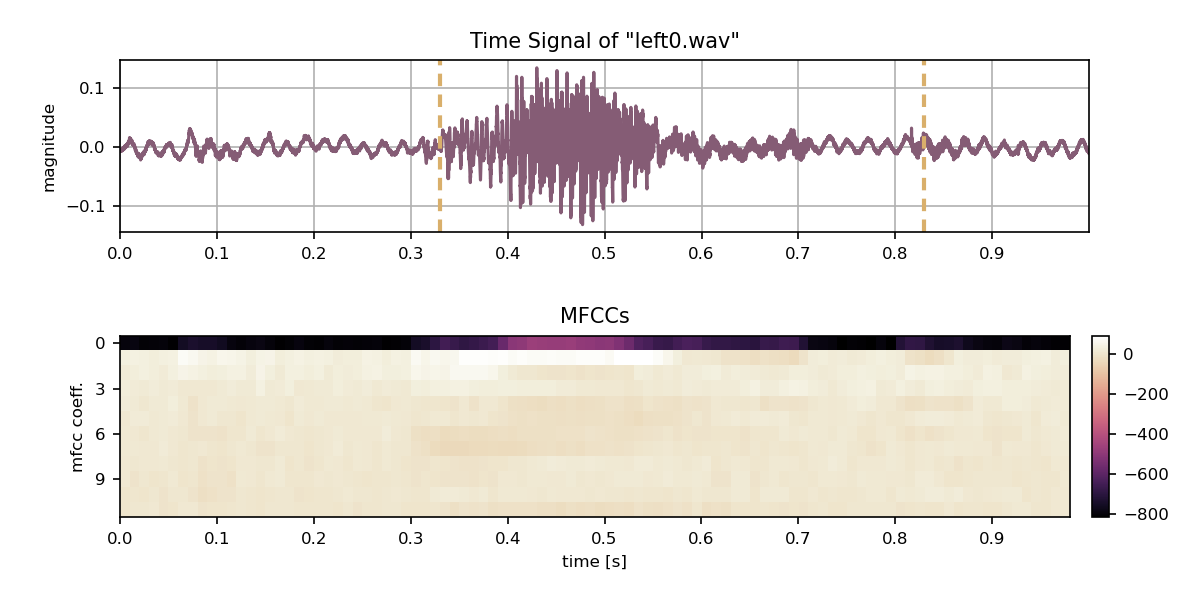
\includegraphics[width=0.75\textwidth]{./3_theory/figs/a3_mfcc/left0_mfcc_only.png}
  \caption{Bad visualisation of the 12 MFCCs features extracted from \enquote{left0.wav}.}
  \label{fig:left0_mfcc_only}
\end{figure}
\FloatBarrier
\noindent
Not much structure of the MFCCs can be seen here, due to the vast value difference of the first coefficient. At least the first coefficient shows, where the center of signal energy is placed on the time scale, but other than that, this visualisation is worthless.
Another very bad visualisation is shown by computing the 39 MFCC feature vectors (with Deltas, Double Deltas and Energies) in \rfig{left0_no_order}.

\begin{figure}[!ht]
  \centering
    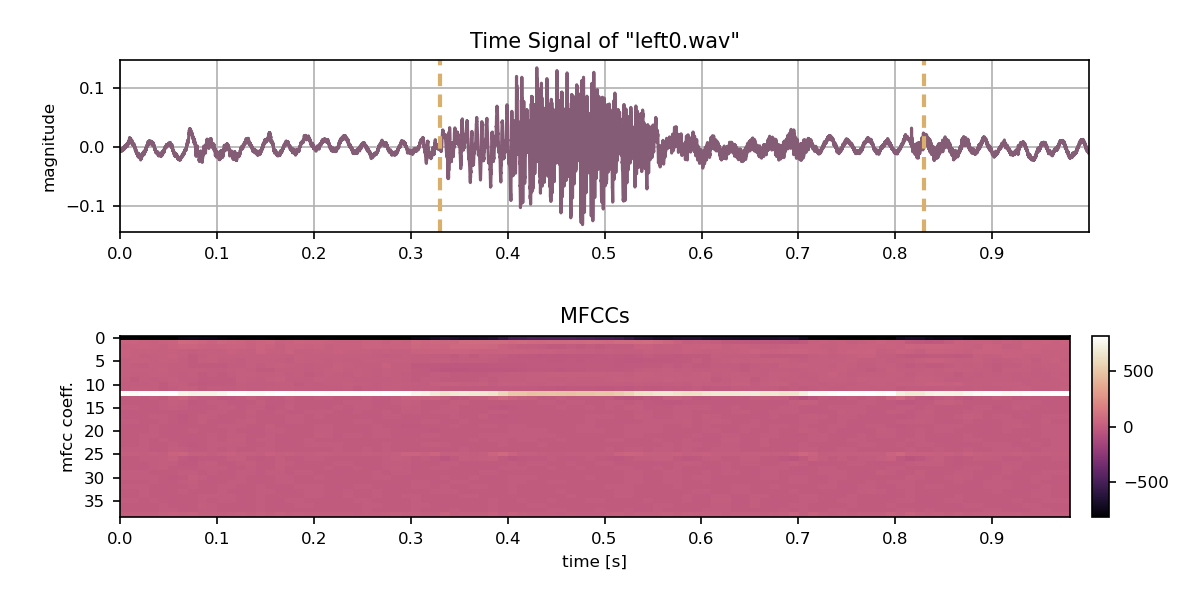
\includegraphics[width=0.75\textwidth]{./3_theory/figs/a3_mfcc/left0_no_order_norm0.png}
  \caption{Very bad visualisation of 39 MFCC features extracted from \enquote{left0.wav}.}
  \label{fig:left0_no_order}
\end{figure}
\FloatBarrier
\noindent
There appears an even greater gap of different value spaces and even less is seen.
One very easy solution is to show the features in different value groups. For instance the first coefficient and its deltas is in one group, the other coefficients in another and the deltas and energies are separated as well in own groups. Now we actually can see some structure in the visualisations, shown in \rfig{left0_order}.

\begin{figure}[!ht]
  \centering
    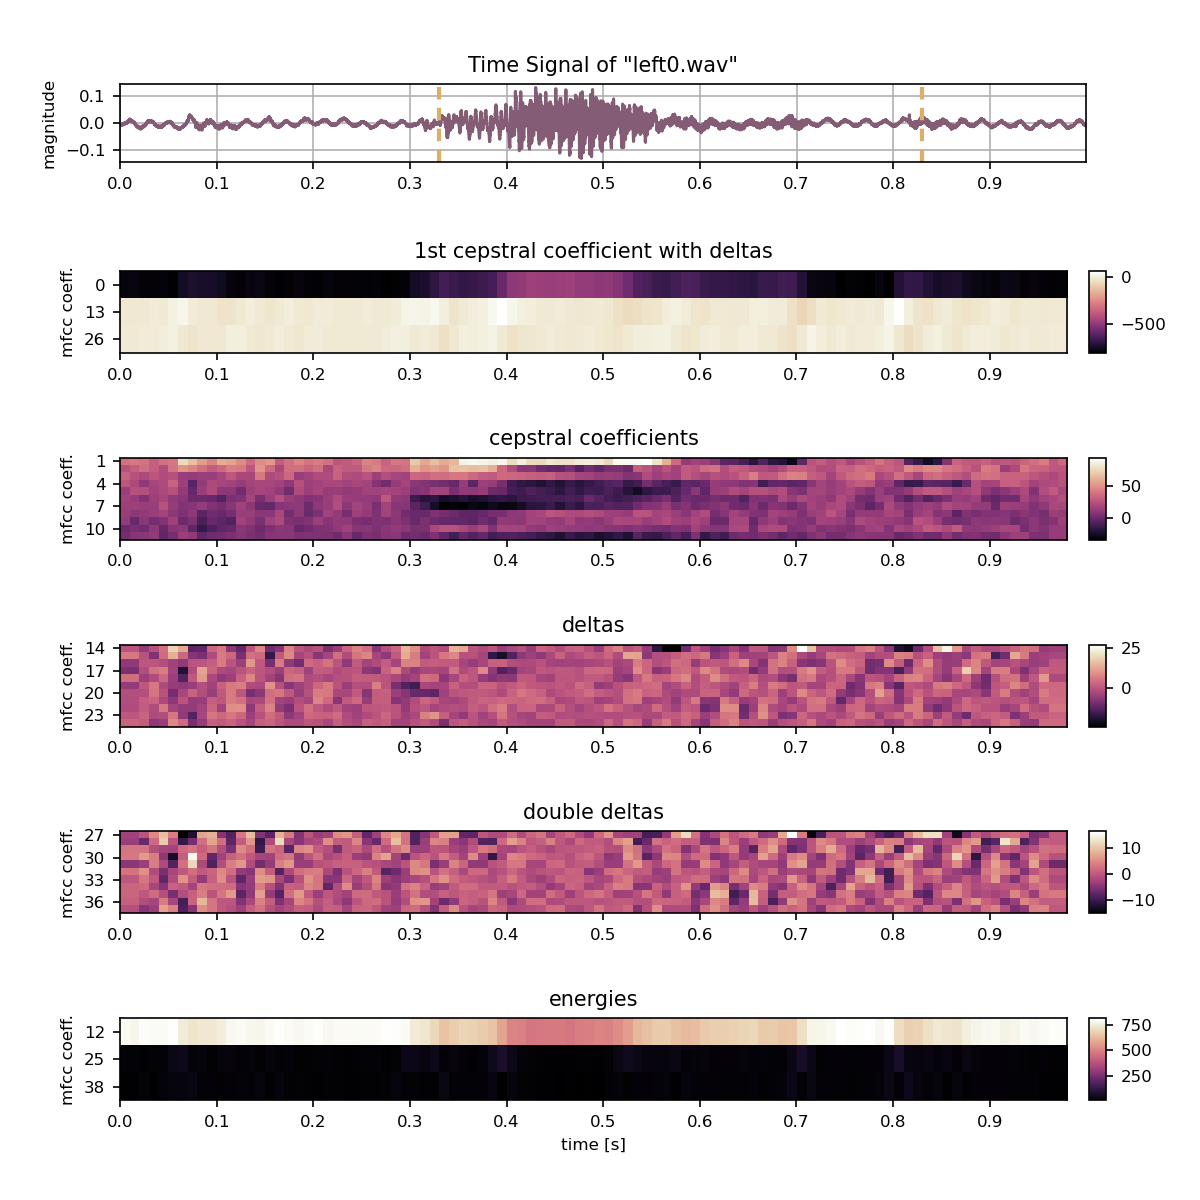
\includegraphics[width=0.75\textwidth]{./3_theory/figs/a3_mfcc/left0_norm0.png}
  \caption{Good visualisation of 39 MFCC features extracted from \enquote{left0.wav} with own value groupings.}
  \label{fig:left0_order}
\end{figure}
\FloatBarrier
\noindent
Another way to improve the visualisation is to normalize the feature vectors over their each own frame dimension with the infinity norm. This will yield a value space of $[0, 1]$ for each feature vector. With this, the visualisation of the 39 MFCC of \enquote{left0.wav} is shown in \rfig{left0_order},

\begin{figure}[!ht]
  \centering
    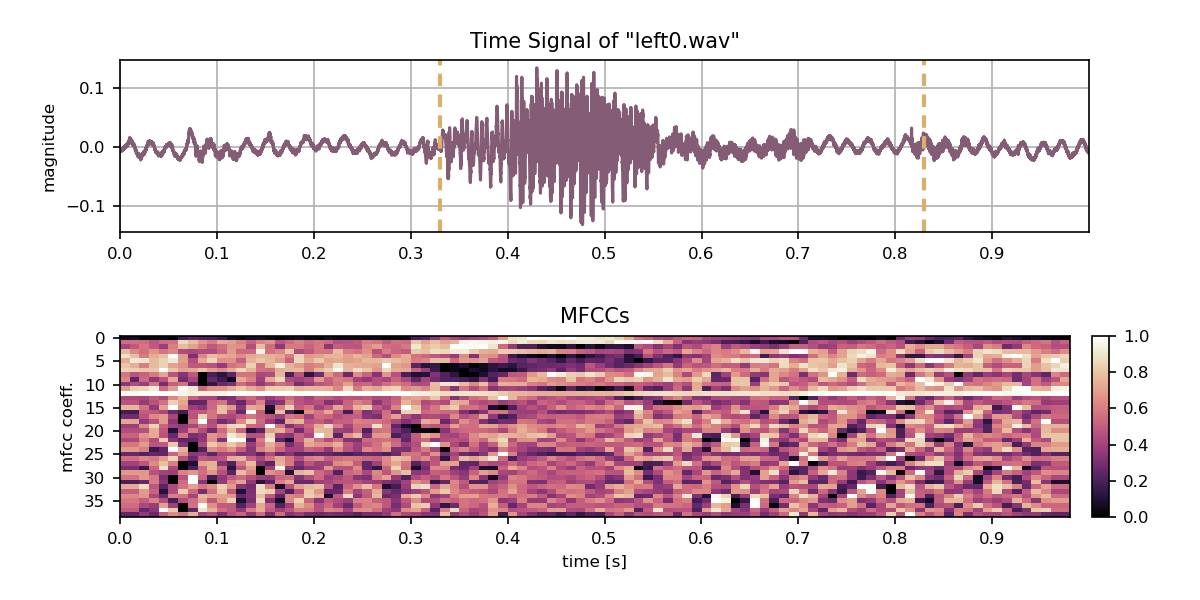
\includegraphics[width=0.75\textwidth]{./3_theory/figs/a3_mfcc/left0_no_order_norm1.png}
  \caption{Normalisation of 39 MFCC features extracted from \enquote{left0.wav}.}
  \label{fig:left0_no_order_norm1}
\end{figure}
\FloatBarrier
\noindent
or in an even better one shown in \rfig{left0_order_norm1}.

\begin{figure}[!ht]
  \centering
    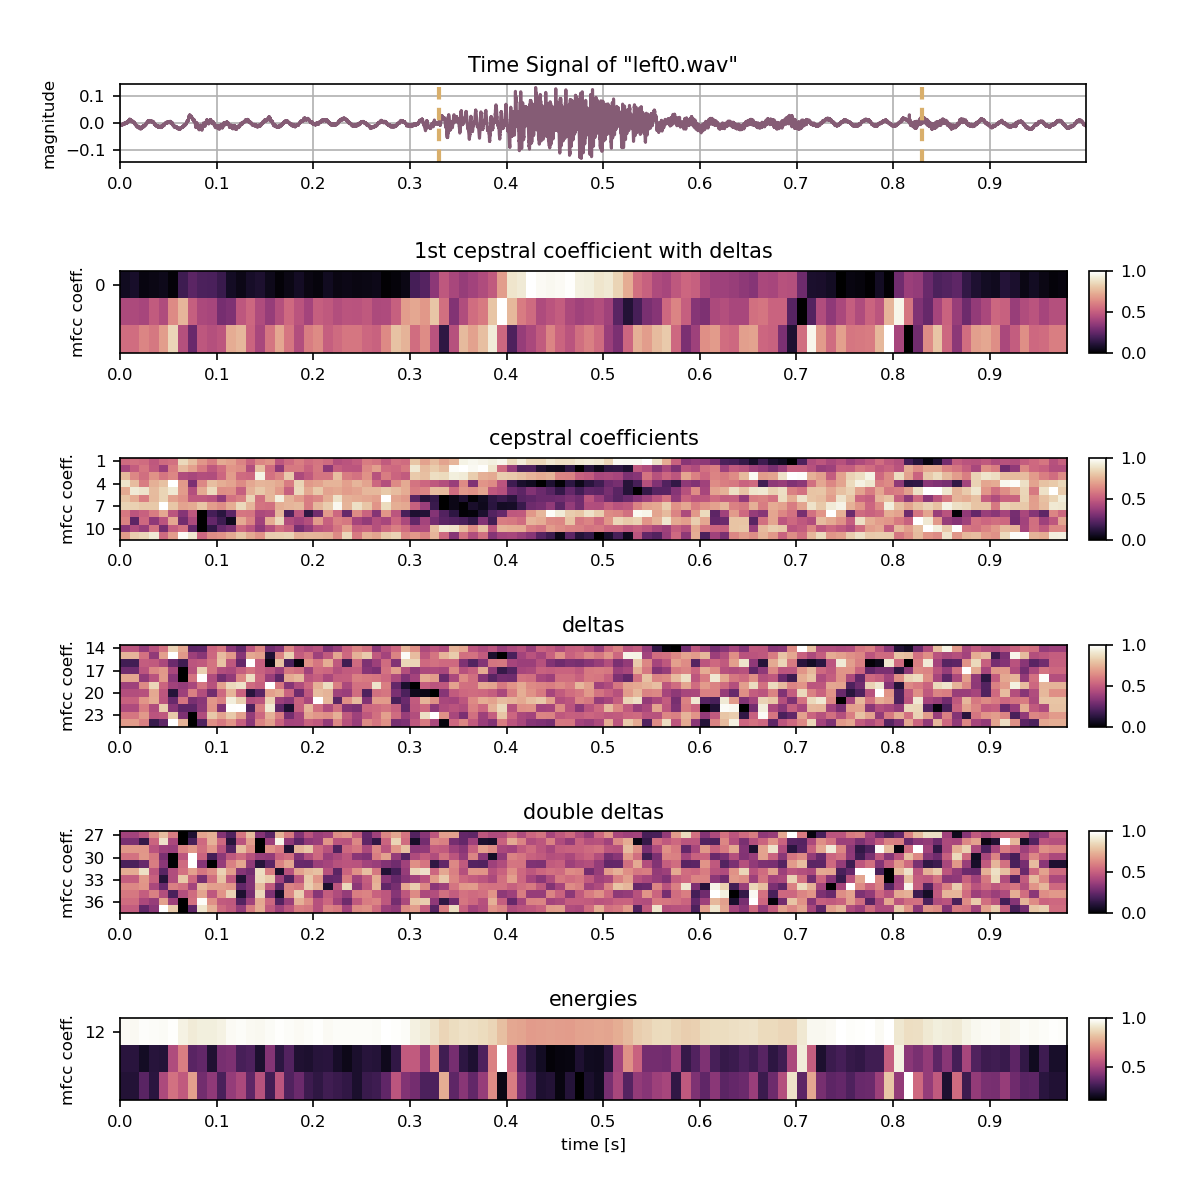
\includegraphics[width=0.75\textwidth]{./3_theory/figs/a3_mfcc/left0_order_norm1.png}
  \caption{Normalisation of 39 MFCC features extracted from \enquote{left0.wav} with groups.}
  \label{fig:left0_order_norm1}
\end{figure}
\FloatBarrier
\noindent
As conclusion, the normalisation in the frame space is an interesting aspect to improve the visualisation of the MFCC features, 
specifically for the cepstral coefficients and the energy features (not the deltas).
Exactly this nice representation was motivating to explore normalisation of feature for Neural Network inputs.
However this is a very crucial thing to do. A normalisation relatives important structures within the feature space and it cannot really be answered if this is a good thing or not.
One more research question arises here: Is it possible to use normalisation for the features as inputs to Neural Networks and what are the results to the accuracy and training of the models.


% ml
\section{Machine Learning Theory}
theory...
\subsection{Neural Network Architectures}\label{sec:nn_arch}
All Neural Network Architectures evaluated within this thesis are presented here.
There will be a general classification between Neural Network Architectures by Convolutional Neural Networks, Adversarial Neural Networks ...
The classification of Convolutional Neural Networks are all Architectures consisting of at least one convolutional layer and the intention to simply classify the speech commands.
As Adversarial Neural Networks we consider Architectures with at least two separate Neural Network Architectures, e.g. a Discriminator and a Generator Network, with the intention to outperform the other Network in a task where they both play a game against each other.
The word game here, is used in the sense of Game Theory, where the goal is to find an equilibrium state where both players are equally satisfied with the state.

% game
\section{Video Game}
Theory?

\chapter{Practice}
The practical part of this thesis can be found in this chapter.
It presents the implementation of the Key Word Spotting system and some Game Design ideas of possible applications with speech commands. 
Further this chapter includes the evolution process of the machine learning approaches used for speech command classification.


% dataset
% --
% dataset

\section{Dataset}
This section discusses the used datasets as input to the machine learning architectures for speech command classification.
The dataset details and properties of the sound files are presented.
Some sound examples and their feature representation of the datasets is shown.
Further the quality and diversity of recorded samples is mentioned.
% --
% Speech Commands dataset

\subsection{Speech Commands Dataset}
The Speech Command Dataset is a very diverse dataset consisting of over thousands of different speakers. This dataset is by any means no clean dataset recorded by professionals, if anything it is the opposite. 
The audio files are not normalized, there are samples with inconsistent sample numbers and some examples are prone with too much noise or even noise only.
And its still great, because there is no need for a perfect dataset and one can be happy that there exists one with this amount of diversity and free of access.
In fact maybe its even better to have an unclean dataset, so that invariances against noise are learnt and do not have be added by hand.
% --
% my dataset

\subsection{My own Dataset}
The author of this thesis recorded some speech command samples by himself and used it as own test set in evaluating trained models in the machine learning part. No self recorded files are used within the training set, so that it can be shown that unseen voice characteristics are classified correctly.

\begin{figure}[!ht]
  \centering
    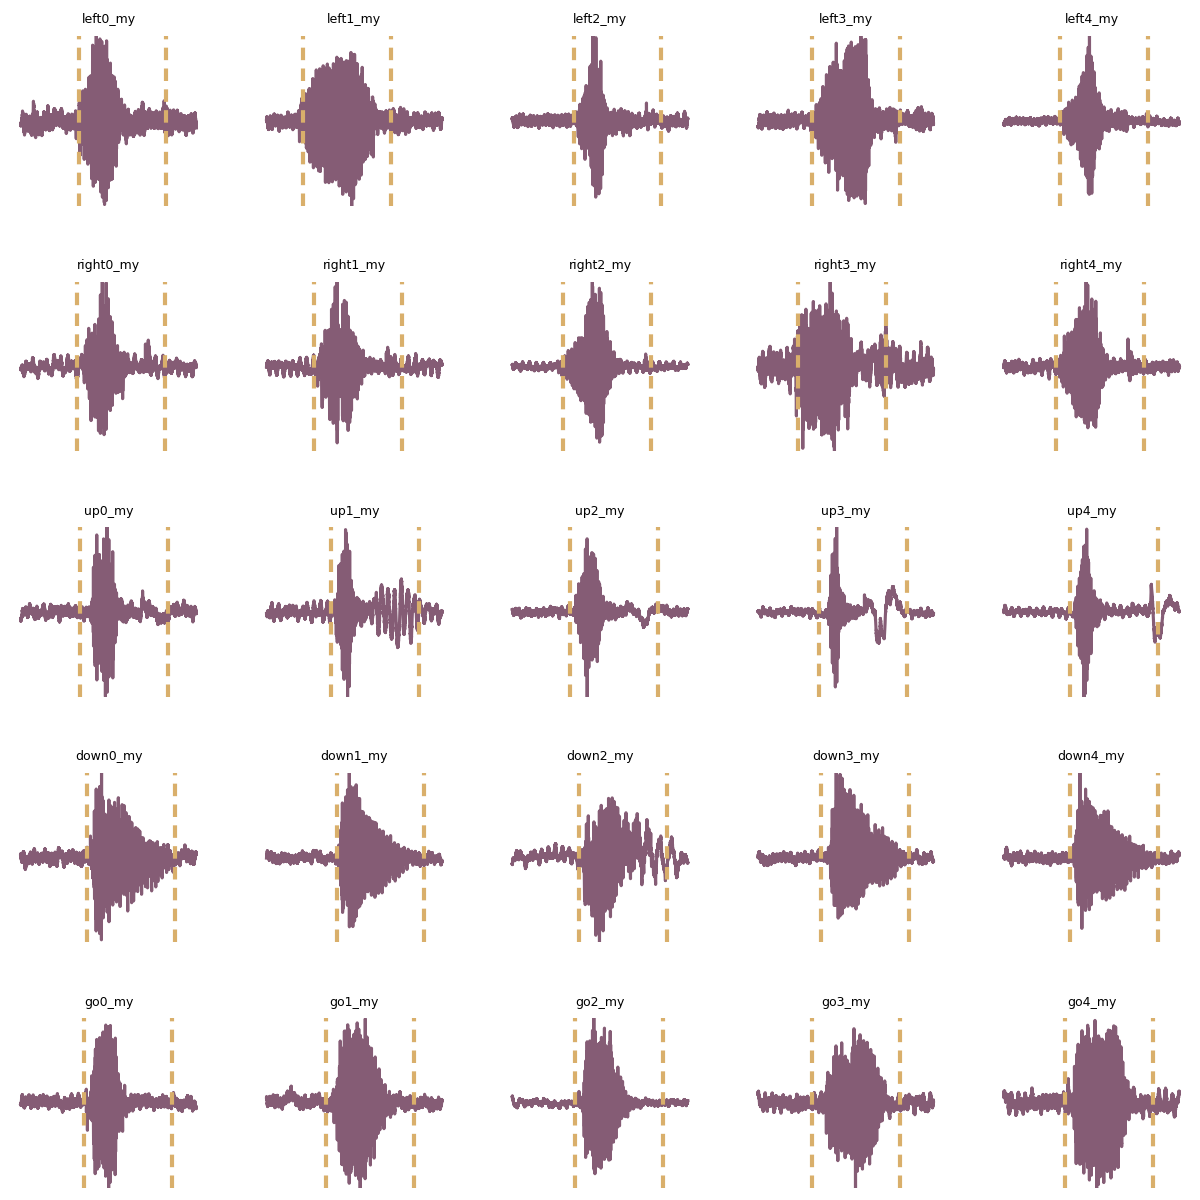
\includegraphics[width=0.65\textwidth]{./4_practice/figs/a_dataset/wav_grid_my}
  \caption{My wav grid}
  \label{fig:wav_grid_my}
\end{figure}
\FloatBarrier
\noindent

% machine learning
\section{Machine Learning}
Machine Learning stuff

% --
% ml details

\subsection{Training Details}
We can separate the training details into three categories:
\begin{enumerate}
  \item Dataset parameters
  \item Features extraction parameters
  \item Feature selection
  \item Machine Learning Training parameters
  \item Transfer Learning parameters
\end{enumerate}
The dataset parameters are the information of what labels from the dataset are used and how many examples per labels.
The feature extraction parameters simply give information about how features are extracted, e.g. this includes the hop size, frame size, filter bands of the MFCC, etc.
The feature selection

\begin{table}[ht!]
\begin{center}
\caption{Dataset Details and References}
\begin{tabular}{ M{2cm}  M{2cm}  M{5cm} }
\toprule
%\multicolumn{4}{c}{\textbf{Feature Groups}} & \multicolumn{2}{c}{\textbf{Accuracy}} \\
\textbf{Reference name} & \textbf{Number of examples per label} & \textbf{Selected Labels}\\
\midrule
500-c5 & 500 & left, right, up, down, go\\
\bottomrule
\end{tabular}
\end{center}
\label{tab:ml_details_dataset}
\end{table}
\FloatBarrier
\noindent


% --
% feature selection

\subsection{Feature Selection}
Now that the Neural Network Architectures are described in \rsec{nn_arch} and basic knowledge about MFCCs is given in \rsec{features} it is important to evaluate the impact of the selection of certain MFCC feature constellations to the accuracy of the Test sets.
In detail it is shown how a fixed model is trained with features consisting of following MFCC parts:
\begin{enumerate}
    \item Cepstral Coefficients (usual MFCCs)
    \item Deltas (frame difference of MFCCs)
    \item Double Deltas (frame difference of Deltas)
    \item Energy Vector (added to each of the upper features)
\end{enumerate}
Another crucial point is to evaluate whether a frame based normalization of these features hurt the training and the accuracy of the models.

\begin{table}[ht!]
\begin{center}
\caption{Feature Selection ml it500 c5 features fc1}
\begin{tabular}{ M{1cm}  M{1cm}  M{1cm}  M{1cm}  M{1.5cm}  M{1.5cm}  M{1.5cm}  M{1.5cm} }
\toprule
\multicolumn{4}{c}{\textbf{Feature Groups}} & \multicolumn{2}{c}{\textbf{Accuracy}} \\
\textbf{c} & \textbf{d} & \textbf{dd} & \textbf{e} & \textbf{acc test} & \textbf{acc my} & \textbf{acc test norm} & \textbf{acc my norm} \\
\midrule
0 & 0 & 1 & 0 & 86.67 & 80.00 & 68.33 & 73.33 \\
0 & 0 & 1 & 1 & 85.00 & 86.67 & 67.67 & 73.33 \\
0 & 1 & 0 & 0 & 92.67 & 100.00 & 75.67 & 80.00 \\
0 & 1 & 0 & 1 & 90.67 & 90.00 & 82.00 & 73.33 \\
0 & 1 & 1 & 0 & 91.00 & 93.33 & 76.67 & 70.00 \\
0 & 1 & 1 & 1 & 89.33 & 100.00 & 78.67 & 80.00 \\
1 & 0 & 0 & 0 & 16.67 & 16.67 & 88.33 & 86.67 \\
1 & 0 & 0 & 1 & 33.33 & 33.33 & 86.33 & 80.00 \\
1 & 0 & 1 & 0 & 91.00 & 90.00 & 87.00 & 80.00 \\
1 & 0 & 1 & 1 & 82.67 & 86.67 & 86.67 & 90.00 \\
1 & 1 & 0 & 0 & 91.67 & 76.67 & 88.33 & 90.00 \\
1 & 1 & 0 & 1 & 90.00 & 80.00 & 89.33 & 93.33 \\
1 & 1 & 1 & 0 & 89.00 & 76.67 & 89.33 & 90.00 \\
1 & 1 & 1 & 1 & 88.00 & 90.00 & 89.00 & 86.67 \\
\bottomrule
\end{tabular}
\end{center}
\label{tab:ml_it500_c5_features_fc1}
\end{table}
\FloatBarrier
\noindent


\begin{table}[ht!]
\begin{center}
\caption{Feature Selection ml it1000 c30 features fc1}
\begin{tabular}{ M{1cm}  M{1cm}  M{1cm}  M{1cm}  M{1.5cm}  M{1.5cm} }
\toprule
\multicolumn{4}{c}{\textbf{Feature Groups}} & \multicolumn{2}{c}{\textbf{Accuracy}} \\
\textbf{c} & \textbf{d} & \textbf{dd} & \textbf{e} & \textbf{acc test} & \textbf{acc test norm} \\
\midrule
0 & 0 & 1 & 0 & 52.97 & 33.10 \\
0 & 0 & 1 & 1 & 56.65 & 27.94 \\
0 & 1 & 0 & 0 & 63.55 & 39.68 \\
0 & 1 & 0 & 1 & 74.52 & 48.65 \\
0 & 1 & 1 & 0 & 71.03 & 39.35 \\
0 & 1 & 1 & 1 & 73.94 & 46.39 \\
1 & 0 & 0 & 0 & 47.23 & 58.19 \\
1 & 0 & 0 & 1 & 45.35 & 57.81 \\
1 & 0 & 1 & 0 & 60.45 & 47.55 \\
1 & 0 & 1 & 1 & 59.48 & 51.61 \\
1 & 1 & 0 & 0 & 58.77 & 55.10 \\
1 & 1 & 0 & 1 & 6.45 & 47.81 \\
1 & 1 & 1 & 0 & 65.81 & 60.39 \\
1 & 1 & 1 & 1 & 62.06 & 51.55 \\
\bottomrule
\end{tabular}
\end{center}
\label{tab:ml_it1000_c30_features_fc1}
\end{table}
\FloatBarrier
\noindent



\section{Adversarial Training}
Adversarial is great

% game design
\section{Video Game}
Theory?




\chapter{Formulary}
All formulars used within this thesis are presented here.
Fourier-Transform (FT):
\begin{equation}
    X(\omega) = \int_{-\infty}^\infty x(t) \, e^{-j 2 \pi \omega t} \,dt
\end{equation}
\noindent
Discrete Fourier-Transform (DFT):
\begin{equation}
    X[k] = \sum_{n=0}^{N-1} x[n] \, e^{-j\frac{2 \pi n}{N}k}
\end{equation}
which can be conveniently written in Matrix form:
\begin{equation}
    X[k] = D\, x[n] \quad \mathrm{with} 
    \quad D[p, q] = e^{-j\frac{2 \pi p}{N} q},
    \quad p, q = 0 \dots N-1
\end{equation}
Short-time Fourier transform (STFT) for discrete time signals:
\begin{equation}
    X(m, \omega) = \sum_{n=-\infty}^{\infty} x[n] \, w[n-m] e^{-j\omega n}
\end{equation}


% --
% bib

% print bib
\printbibliography[heading=bibintoc]


\end{document}